
%%%%%%%%%%%%%%%%%%%%%%% file typeinst.tex %%%%%%%%%%%%%%%%%%%%%%%%%
%
% This is the LaTeX source for the instructions to authors using
% the LaTeX document class 'llncs.cls' for contributions to
% the Lecture Notes in Computer Sciences series.
% http://www.springer.com/lncs       Springer Heidelberg 2006/05/04
%
% It may be used as a template for your own input - copy it
% to a new file with a new name and use it as the basis
% for your article.
%
% NB: the document class 'llncs' has its own and detailed documentation, see
% ftp://ftp.springer.de/data/pubftp/pub/tex/latex/llncs/latex2e/llncsdoc.pdf
%
%%%%%%%%%%%%%%%%%%%%%%%%%%%%%%%%%%%%%%%%%%%%%%%%%%%%%%%%%%%%%%%%%%%


\documentclass[runningheads,a4paper,orivec]{llncs}

\usepackage{amssymb,amsmath}
\setcounter{tocdepth}{3}
\usepackage{graphicx}
\usepackage[ruled,linesnumbered]{algorithm2e}

\usepackage{url}
\urldef{\mailsa}\path|{yingqin,syshen,|
\urldef{\mailsb}\path|huadongdai,|
\urldef{\mailsc}\path|qingbowu,yanjia}@nudt.edu.cn|
\newcommand{\keywords}[1]{\par\addvspace\baselineskip
\noindent\keywordname\enspace\ignorespaces#1}

% \newtheorem{algorithm}{Algorithm}

\begin{document}

\mainmatter  % start of an individual contribution

% first the title is needed
%\title{Lecture Notes in Computer Science:\\Authors' Instructions
%for the Preparation\\of Camera-Ready
%Contributions\\to LNCS/LNAI/LNBI Proceedings}
\title{Complementary Synthesis for Encoders with Pipeline and Flow Control Mechanism}

% a short form should be given in case it is too long for the running head
%\titlerunning{Lecture Notes in Computer Science: Authors' Instructions}

% the name(s) of the author(s) follow(s) next
%
% NB: Chinese authors should write their first names(s) in front of
% their surnames. This ensures that the names appear correctly in
% the running heads and the author index.
%
\author{Ying Qin %
%\thanks{Project 61070132 supported by National Natural Science Foundation of China.}%
\and ShengYu Shen \and HuaDong Dai \and QingBo Wu \and Yan Jia}
%
\authorrunning{Ying Qin %
\and ShengYu Shen \and HuaDong Dai \and QingBo Wu \and Yan Jia}
% (feature abused for this document to repeat the title also on left hand pages)

% the affiliations are given next; don't give your e-mail address
% unless you accept that it will be published
\institute{School of Computer, National University of Defense Technology, China\\
\mailsa\mailsb\mailsc\\
% \url{}
}

%
% NB: a more complex sample for affiliations and the mapping to the
% corresponding authors can be found in the file "llncs.dem"
% (search for the string "\mainmatter" where a contribution starts).
% "llncs.dem" accompanies the document class "llncs.cls".
%

\toctitle{Lecture Notes in Computer Science}
\tocauthor{Authors' Instructions}
\maketitle


\begin{abstract}
Complementary synthesis automatically generates an encoder's decoder
that recovers the encoder's inputs from its output,
even if this encoder contains flow control mechanism that prevents
its inputs from being uniquely determined by its outputs.
At the same time,
most encoders also include pipeline stages that can be exploited to improve the decoder's timing.
\vspace{0.1cm}

This paper proposes a novel algorithm to handle encoders with both pipeline and flow control mechanism.
First,
it infers the flow control predicate on inputs with state-of-the-art algorithm.
Second,
it finds out the pipeline stages in the encoder by enforcing the inferred flow control predicate.
Third,
it infers the flow control predicate for each pipeline stages.
Finally,
the decoder's Boolean functions that recover each pipeline stage and input are characterized with Craig interpolant.

\vspace{0.1cm}

Experimental results on several complex encoders indicate that
this algorithm can always correctly generate a pipelined decoders with inferred flow control mechanism.

\keywords{Complementary Synthesis, Flow Control Mechanism, Pipeline Stage, Craig Interpolation}
\end{abstract}


\section{Introduction}\label{sec_intro}
One of the most difficult jobs in designing communication
and multimedia chips is to design and verify complex encoder and decoder pairs.
The encoder maps its input variables $\vec{i}$ to its output variables $\vec{o}$,
% according to some predefined rules,
% such as Ethernet \cite{IEEE8023_S4} and PCI Express \cite{pcie21},
while the decoder recovers $\vec{i}$ from $\vec{o}$.
Complementary synthesis 
\cite{ShenICCAD09,ShenTCAD11,ShenTCAD12,LiuICCAD11,LiuTCAD12,TuDAC13}
eases this job by
automatically generating a decoder from an encoder,
with the assumption that $\vec{i}$ can always be
uniquely determined by a bounded sequence of $\vec{o}$.
% Thus,
% the decoder's Boolean function can be characterized
% with the algorithm proposed by Jiang et al. \cite{InterpBoolFunction}
% This algorithm constructs an unsatisfiable formula with two unrolled transition function sequences,
% both of which have the same output sequence but with different input.
% A Craig interpolant \cite{Craig} can be extracted from this unsatisfiable formula,
% and used as the decoder's Boolean function that recovers the inputs.

However,
the flow control mechanism \cite{flowcontrol} widely employed in many encoders
fails this assumption.
It prevents faster transmitter from overwhelming slower receiver,
by transmitting idle symbols that can only uniquely determine a small subset of inputs instead of valid data,
when the receiver can't keep up with the transmitter.
We call such inputs the flow control vector $\vec{f}$,
and other inputs the data vector $\vec{d}$.

\begin{figure}[t]
\centering
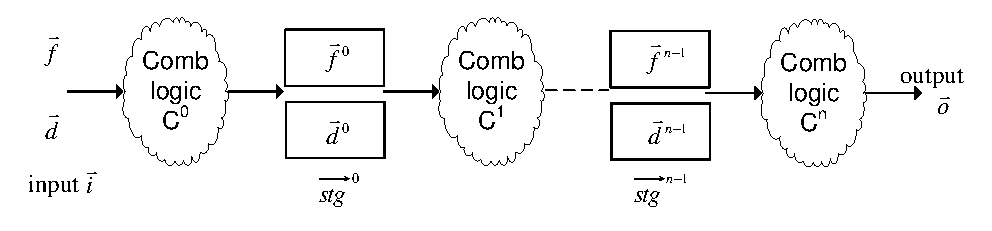
\includegraphics[width=\textwidth]{pipemod1}
\caption{Encoder with pipeline and flow control mechanism}
\label{pipemod}
\end{figure}

Qin et al. \cite{QinTODAES15} handle such encoders by
first finding out all inputs $i\in\vec{i}$ that can by uniquely determined by $\vec{o}$,
and taking them as $\vec{f}$,
and then inferring a predicate $valid(\vec{f})$ that,
when enforced,
can make $\vec{d}$ to be uniquely determined by $\vec{o}$.

At the same time,
as shown in Figure \ref{pipemod},
many encoders contain
pipeline stages $\vec{stg}^j$ to cut their datapath into multiple segments $C^j$,
such that the encoder can run in higher frequency.
But the decoder generated by Qin et al. \cite{QinTODAES15} does not include pipeline stages,
which make it much slower than the corresponding encoder.

To overcome this problem,
this paper proposes a novel algorithm to generate pipelined decoders for flow controlled encoder.
It first apply Qin et al. \cite{QinTODAES15}'s algorithm to find out $\vec{f}$ and infers $valid(\vec{f})$ that can make $\vec{d}$ to be uniquely 
determined by $\vec{o}$.
By assuming that each pipeline stage $\vec{stg}^j$ can be partitioned into flow control vector $\vec{f}^j$ and data vector $\vec{d}^j$,
this algorithm then finds out $\vec{d}^j$ and $\vec{f}^j$ respectively with and without enforcing $valid(\vec{f})$.
It finally characterize the Boolean function that recover each $\vec{stg}^j$ and $\vec{i}$ with 
Jiang et al. \cite{InterpBoolFunction}'s algorithm.

\emph{The remainder of this paper is organized as follows}.
%Section \ref{sec_casestudy} explains our ideas with a simple example.
Section \ref{sec_prem} introduces the background material;
% Section \ref{sec_findfc} identifies the flow control variables,
% and infers the predicate that enables $\vec{d}$ 
% to be uniquely determined by a bounded sequence of $\vec{o}$;
Section \ref{sec_pipe} finds out the pipeline stages $\vec{stg}^j$,
while Section \ref{sec_pred} infers  $valid^j(\vec{stg}^j)$ for each pipeline stage and input vector $\vec{i}$;
Section \ref{sec_char} characterize the decoder's Boolean functions that recover each pipeline stage $\vec{stg}^j$ and the input vector $\vec{i}$.
Sections \ref{sec_exp} and \ref{sec_relwork} present the experimental results and related works;
Finally,
Section \ref{sec_conclude} sums up the conclusion.

\section{Preliminaries}\label{sec_prem}

% \subsection{Flow control mechanism}\label{subsec_fc}



\subsection{Propositional satisfiability}\label{subsec_SAT}
% We use a denotation similar to that of \cite{TuDAC13}.
The Boolean value set is denoted as $B=\{0,1\}$.
A vector of variables is represented as $\vec{v}=(v,\dots)$.
The number of variables in $\vec{v}$ is denoted as $|\vec{v}|$.
If a variable $v$ is a member of $\vec{v}$,
% that is $\vec{v}=(\dots,v,\dots)$,
then we say $v\in\vec{v}$;
otherwise we say $v\notin\vec{v}$.
For a variable $v$ and a vector $\vec{v}$,
if $v\notin\vec{v}$,
then the new vector that contains both $v$ and all members of $\vec{v}$ is denoted as $v\cup\vec{v}$.
If $v\in \vec{v}$,
then the new vector that contains all members of $\vec{v}$ except $v$,
is denoted as $\vec{v}-v$.
For the two vectors $\vec{a}$ and $\vec{b}$,
the new vector with all members of $\vec{a}$ and $\vec{b}$ is denoted as $\vec{a}\cup\vec{b}$.
The set of truth valuations of $\vec{v}$ is denoted as $[\![\vec{v}]\!]$,
for instance,
$[\![(v_1,v_2)]\!]=\{(0,0),(0,1),(1,0),(1,1)\}$.

% A Boolean formula $F$ over a variable set $V$ is constructed by connecting variables from $V$ 
% with symbols $\neg$, $\wedge$, $\vee$ and $\Rightarrow$,
% which stand for logical connectives negation, conjunction, disjunction, and implication, respectively.

The propositional satisfiability problem(abbreviated as SAT) for a Boolean formula $F$ over a variable set $V$ 
is to find a satisfying assignment $A:V\to B$,
so that $F$ can be evaluated to $1$.
If $A$ exists, then $F$ is satisfiable;
otherwise,
it is unsatisfiable.

% A computer program that decides the existence of such a satisfying assignment is called a SAT solver,
%  such as Zchaff\cite{CHAFF},
%  Grasp\cite{grasp},
%  Berkmin\cite{BERKMIN},
%  and MiniSat\cite{EXTSAT}.
 
% Normally,
% a SAT solver requires the formula to be represented in the conjunctive normal form(CNF),
% in which a formula is a conjunction of its clause set,
% and a clause is a disjunction of its literal set,
% and a literal is a variable or its negation.
% A formula in the CNF format is also called a SAT instance,


% \subsection{Cofactoring}\label{subsec_pre_cofact}

% For a Boolean function $f:B^n\to B$,
% we use $supp(f)$ to denote its support set $\{v_1\dots v_n\}$.
According to \cite{EFFSATUSMCCO},
the positive and negative cofactors of $f(v_1\dots v\dots v_n)$ with respect to variable
$v$ are $f_{v\equiv 1}=f(v_1\dots 1\dots v_n)$ and $f_{v\equiv 0}=f(v_1\dots 0\dots v_n)$,
respectively.
% Existential quantification of $f(v_1\dots v\dots v_n)$ with respect to a
% variable $v$ is $\exists v f=f_v+f_v’$.
\textbf{Cofactoring} is the action that applies 1 or 0 to $v$ to get $f_{v\equiv 1}$ or $f_{v\equiv 0}$.

% \subsection{Craig interpolation}\label{subsec_pre_interp}
% Craig\cite{Craig} had proved the following theorem:
% \begin{theorem}[Craig Interpolation Theorem\cite{Craig}]\label{thm_craig}
Given two Boolean formulas $\phi_A$ and $\phi_B$,
with $\phi_A\wedge \phi_B$ unsatisfiable,
there exists a formula $\phi_I$ referring only
to the common variables of $\phi_A$ and $\phi_B$ such that $\phi_A\Rightarrow \phi_I$
and $\phi_I\wedge \phi_B$ is unsatisfiable.
We call $\phi_I$ the \textbf{interpolant} \cite{Craig} of $\phi_A$ with respect to $\phi_B$
% \end{theorem}
and use McMillan's algorithm \cite{interp_McMillan} to generate it.




\subsection{Finite state machine}\label{subsec_fsm}



The encoder is modeled by a finite state machine(FSM) $M=(\vec{s},\vec{i},\vec{o},T)$,
consisting of a state variable vector $\vec{s}$,
% an initial state $s_0\in S$,
an input variable vector $\vec{i}$,
% a finite set of configuration letters $C$,
an output variable vector $\vec{o}$,
and a transition function $T: [\![\vec{s}]\!]\times [\![\vec{i}]\!]\to [\![\vec{s}]\!]\times [\![\vec{o}]\!]$ 
that computes the next state and output variable vector from the current state and input variable vector.

% As shown in Figure \ref{mealy},
% as well as in the remainder of this paper,
% the state is represented as a gray round corner box,
% and the transition function $T$ is represented as a white rectangle.
The behavior of FSM $M$ can be reasoned by unrolling transition function for multiple steps.
The state variable $s\in\vec{s}$, input variable $i\in\vec{i}$ and output variable $o\in\vec{o}$ at the $n$-th step 
are respectively denoted as $s_n$, $i_n$ and $o_n$.
Furthermore,
the state, the input and the output variable vectors at the $n$-th step are respectively denoted as $\vec{s}_n$, $\vec{i}_n$ and $\vec{o}_n$.
% We further denote the sequence of state, input letter and output letter from the $n$-th to the $m$-th step respectively as $s_n^m$, $i_n^m$ and $o_n^m$.
A \textbf{path} is a state sequence $<\vec{s}_n,\dots,\vec{s}_m>$ with $\exists \vec{i}_j\vec{o}_j (\vec{s}_{j+1},\vec{o}_j)\equiv T(\vec{s}_j,\vec{i}_j)$ for all $n\le j< m$.
A \textbf{loop} is a path $<\vec{s}_n,\dots,\vec{s}_m>$ with $\vec{s}_n\equiv \vec{s}_m$.



\subsection{The halting algorithm to find out flow control vector $\vec{f}$}\label{subsec_chkextdec}


Qin et al. \cite{QinTODAES15} proposed the first halting algorithm
to infer flow control predicates by iteratively unrolling the transition function.
And for each iteration,
it uses two approximative approaches to determine the answer.
The first one is an under-approximative one that presented in \ref{subsub_sound},
while the second one is an over-approximative one presented in \ref{subsub_complete}.
And we will show in \ref{subsubsec_findfc} that these two approaches will eventually converge.

\subsubsection{The under-approximative approach}\label{subsub_sound}.

As shown in Figure \ref{fig_pc}a),
on the unrolled transition functions,
an input variable $i\in\vec{i}$ can be uniquely determined,
if there exist three integers $p$, $l$ and $r$,
such that for any particular valuation of the output sequence $<\vec{o}_p,\dots,\vec{o}_{p+l+r}>$,
$i_{p+l}$ cannot be 0 and 1 at the same time.
This is equal to the unsatisfiability of $F_{PC}(p,l,r)$ in Equation (\ref{uniqt1}).

\begin{equation}\label{uniqt1}
% \begin{split}
F_{PC}(p,l,r):=
\left\{
\begin{array}{cc}
&\bigwedge_{m=0}^{p+l+r}
\{
(\vec{s}_{m+1},\vec{o}_m)\equiv T(\vec{s}_m,\vec{i}_m)
\}
\\
\wedge&\bigwedge_{m=0}^{p+l+r}
\{
(\vec{s'}_{m+1},\vec{o'}_m)\equiv T(\vec{s'}_m,\vec{i'}_m)
\}
\\
\wedge&\bigwedge_{m=p}^{p+l+r}\vec{o}_m\equiv \vec{o'}_m \\
\wedge& i_{p+l}\equiv 1 \wedge  i'_{p+l}\equiv 0 
% \wedge&\bigwedge_{m=0}^{p+l+r}assertion(\vec{i}_m) \\
% \wedge&\bigwedge_{m=0}^{p+l+r}assertion(\vec{i'}_m) 
\end{array}
\right\}
% \end{split}
\end{equation}

\begin{figure}[t]
\begin{center}
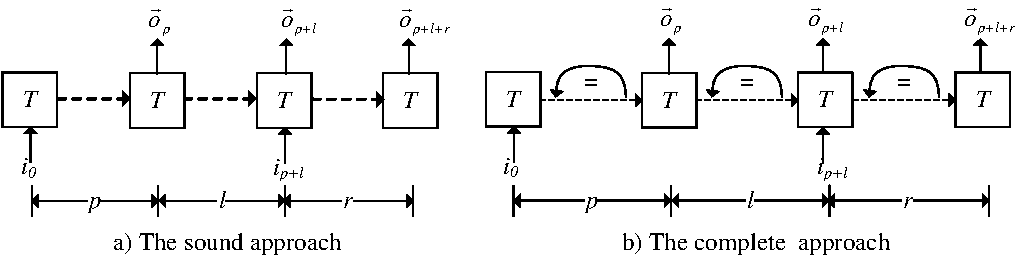
\includegraphics[width=\textwidth]{pc}
\end{center}
\caption{The under and over-approximative approaches}
  \label{fig_pc}
\end{figure}


Here,
$p$ is the length of the prefix state transition sequence.
$l$ and $r$ are the lengths of the two output sequences 
$<\vec{o}_{p+1},\dots,\vec{o}_{p+l}>$ and $<\vec{o}_{p+l+1},\dots,\vec{o}_{p+l+r}>$
used to determine $i_{p+l}$.
Line 1 of Equation (\ref{uniqt1}) corresponds to the left path in Figure \ref{fig_pc}a),
while Line 2 corresponds to the right path in Figure \ref{fig_pc}a).
These two paths are of the same length.
Line 3 forces these two paths' output sequences to be the same,
while Line 4 forces their $i_{p+l}$ to be different.
% Line 5 and 6 are the assertion predicates given 
% by the user that constrain the valid valuation on $\vec{i}$.
% PC in $F_{PC}$ is the abbreviation of "parameterized complementary",
% which means $F_{PC}(p,l,r)$ is used to check whether the encoder's input can be uniquely determined with the three parameters $p$, $l$ and $r$.


According to Figure \ref{fig_pc}a),
the first three lines of Equation (\ref{uniqt1}) are two unrolled transition function sequences with the same output sequences.
They can always be satisfied with the same input variable vectors and initial state vector.
And the last two lines are constraints on input variable vectors.
We always check their satisfiability before running our algorithm.
So the unsatisfiability of $F_{PC}(p,l,r)$ always means $i_{p+l}\equiv i'_{p+l}$.


% According to Figure \ref{fig_pc},
% % it is obvious that,
% if $F_{PC}(p,l,r)$ is unsatisfiable,
% then $F_{PC}(p',l',r')$ is also unsatisfiable for $p'\ge p$, $l'\ge l$ and $r'\ge r$.
According to Equation (\ref{uniqt1}),
% and Figure \ref{fig_pc},
% we can find that,
for $p'\ge p$, $l'\ge l$ and $r'\ge r$,
the clause set of $F_{PC}(p',l',r')$ is a super set of $F_{PC}(p,l,r)$.
% This also lead to the same conclusion.
% This means,
So,
the bounded proof of $F_{PC}(p,l,r)$'s unsatisfiability
can be generalized to unbounded cases.

\begin{proposition}\label{prop_pc1}
If $F_{PC}(p,l,r)$ is unsatisfiable,
% then $i_{p+l}$ cannot take on two different values for any particular valuation of the output sequence $<\vec{o}_{p},\dots,\vec{o}_{p+l+r}>$,
then $i_{p+l}$ can be uniquely determined by $<\vec{o}_{p},\dots,\vec{o}_{p+l+r}>$ for all larger $p$, $l$ and $r$.
\end{proposition}



\subsubsection{The over-approximative approach}\label{subsub_complete}.

For $F_{PC}(p,l,r)$ presented in last subsection,
there are two possibilities:
\begin{enumerate}
 \item 
$i_{p+l}$ can be uniquely determined by $<\vec{o}_{p},\dots,\vec{o}_{p+l+r}>$ for some $p$, $l$ and $r$;
 \item 
$i_{p+l}$ can't be uniquely determined by $<\vec{o}_{p},\dots,\vec{o}_{p+l+r}>$ for any $p$, $l$ and $r$ at all.
\end{enumerate}

If it is the 1st case,
then by iteratively increasing  $p$, $l$ and $r$,
$F_{PC}(p,l,r)$ will eventually become unsatisfiable.
But if it is the 2nd case,
this method will never terminate.

% \begin{figure}[t]
% \begin{center}
% 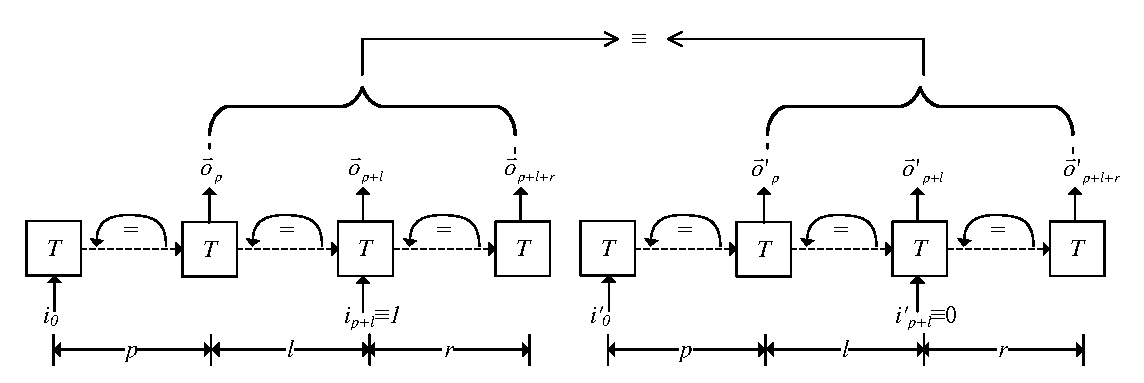
\includegraphics[width=\textwidth]{ln}
% \end{center}
% \caption{The over-approximative  approach checking if $i_{p+l}$ can NOT be uniquely determined}
%   \label{fig_ln}
% \end{figure}

So,
to obtain a halting algorithm,
we need to distinguish these two cases.
One such solution is shown in Figure \ref{fig_pc}b),
which is similar to Figure \ref{fig_pc}a) but with three additional constraints used to detect loops 
on the three state sequences $<\vec{s}_{0},\dots,\vec{s}_{p}>$,$<\vec{s}_{p+1},\dots,\vec{s}_{p+l}>$ and 
$<\vec{s}_{p+l+1},\dots,\vec{s}_{p+l+r}>$.
It is formally defined in Equation (\ref{uniqln}) with the last three lines corresponding to the three new constraints used to detect loops.

\begin{equation}\label{uniqln}
% \begin{split}
F_{LN}(p,l,r):=\\
\left\{
\begin{array}{cc}
&F_{PC}(p,l,r)\\
\wedge&\bigvee_{x=0}^{p-1}\bigvee_{y=x+1}^{p} \{\vec{s}_x\equiv \vec{s}_y\wedge \vec{s'}_x\equiv \vec{s'}_y\} \\
\wedge&\bigvee_{x=p+1}^{p+l-1}\bigvee_{y=x+1}^{p+l} \{\vec{s}_x\equiv \vec{s}_y\wedge \vec{s'}_x\equiv \vec{s'}_y\} \\
\wedge&\bigvee_{x=p+l+1}^{p+l+r-1}\bigvee_{y=x+1}^{p+l+r} \{\vec{s}_x\equiv \vec{s}_y\wedge \vec{s'}_x\equiv \vec{s'}_y\}
\end{array}
\right\}
% \end{split}
\end{equation}

% LN in $F_{LN}$ stands for "loop non-complementary",
% which means $F_{LN}(p,l,r)$ with three loops is used to check whether 
% the input variable can NOT be uniquely determined.


When $F_{LN}(p,l,r)$ is satisfiable,
then $i_{p+l}$ can't be uniquely determined by $<\vec{o}_{p},\dots,\vec{o}_{p+l+r}>$.
More importantly,
by unrolling these three loops,
we can generalize the satisfiability of $F_{LN}(p,l,r)$ to all larger $p$, $l$ and $r$.
This means:


\begin{proposition}\label{prop_ln1}
If $F_{LN}(p,l,r)$ is satisfiable,
then $i_{p+l}$ cannot be uniquely determined by $<\vec{o}_{p},\dots,\vec{o}_{p+l+r}>$ for all larger $p$, $l$ and $r$.
\end{proposition}

\subsubsection{Finding out flow control vector $\vec{f}$}\label{subsubsec_findfc}.

% To facilitate the presentation of our algorithm,
We assume that the input variable vector $\vec{i}$ can be partitioned into 
the flow control vector $\vec{f}$ and the data vector $\vec{d}$.
The flow control vector $\vec{f}$ is used to indicate the validness of $\vec{d}$.
So,
for a properly designed encoder,
$\vec{f}$ should always be uniquely determined by a bounded sequence of the encoder's output vector $\vec{o}$,
or else the decoder cannot recognize the validness of $\vec{d}$.

\begin{algorithm}[t]
\SetAlgoVlined
\KwIn{The input variable vector $\vec{i}$.}
\KwOut{$\vec{f}\subset \vec{i}$ and $\vec{d}\subset \vec{i}$  that can and can't 
be uniquely determined ,and the maximal $p$, $l$ and $r$ reached in this searching.}
$\vec{f}: = \{\}$;$\vec{d}:= \{\}$;$p$:= 0 ;~$l$:= 0 ;~$r$:= 0 \;
\ShowLnLabel{while}\While{$\vec{i}\ne \{\}$}{
  assume $i\in\vec{i}$\;
  $p++$; ~ $l++$; ~ $r++$\;
  \uIf {$F_{PC}(p,l,r)$ is unsatisfiable for $i$} {
    \ShowLnLabel{adduniq}
    $\vec{f}:= i\cup\vec{f}$\;
    $\vec{i}:=\vec{i}-i$\;
  }\ShowLnLabel{nonuniqres}
  \uElseIf {$F_{LN}(p,l,r)$ is satisfiable for  $i$}{
    $\vec{d}:=i\cup\vec{d}$\;
    $\vec{i}:=\vec{i}-i$
  }
}
\KwRet ($\vec{f}$, $p$, $l$, $r$)
\caption{$FindFlow(\vec{i})$:Identifying the flow control vector $\vec{f}$}
\label{alg_fofc}
\end{algorithm}

Thus,
Algorithm \ref{alg_fofc} is proposed to identify $\vec{f}$.
% At Line \ref{initfd},
% the initial value of $f$ and $d$ are set to empty vector.
% At Line \ref{initplr},
% the initial value of $p$, $l$ and $r$ are all set to 0.
At Line \ref{while},
a while loop is used to iterate on all $i\in\vec{i}$.
At Line \ref{adduniq},
the input variable $i$ that can be uniquely determined will be added to vector $\vec{f}$.
On the other hand,
if $F_{LN}(p,l,r)$ is satisfiable at Line \ref{nonuniqres},
the input variable $i$ that can NOT be uniquely determined will be added to vector $\vec{d}$.

Please refer to \cite{QinTODAES15} for details about proving this algorithm's termination and correctness.


\section{Inferring the flow control predicate $valid(\vec{f})$}


% Furthermore,
% the validness of $\vec{d}$ is indicated by a predicate $valid(\vec{f})$.
% So for a properly designed encoder,
% $valid(\vec{f})$ should make $\vec{d}$ to be uniquely determined by the encoder's output.

In Subsection \ref{subsec_craig},
we propose  an algorithm 
to characterize a Boolean function that makes a Boolean formula satisfiable.
In Subsection \ref{subsec_infer},
we apply this algorithm to infer $valid(\vec{f})$,
% the predicate that enable $\vec{d}$ to be uniquely determined by a bounded sequence of $\vec{o}$.
the predicate that enables $\vec{d}$ to be uniquely determined.


\subsection{Characterizing a function that makes a Boolean formula satisfiable}\label{subsec_craig}

For a particular Boolean relation $R(\vec{a},\vec{b},t)$, 
we have the following two assumptions:
\begin{enumerate}
\item \textbf{Assumption 1} :
$R(\vec{a},\vec{b},0)\wedge R(\vec{a},\vec{b},1)$ is unsatisfiable.
% That is,
% $\vec{a}$ and $\vec{b}$ uniquely determine $t$.
$\vec{a}$ and $\vec{b}$ are respectively called the important and the non-important variable vectors,
$t$ is the target variable.
\item \textbf{Assumption 2} :
$R(\vec{a},\vec{b},t)$ is satisfiable for all valuations of $\vec{a}$.
\end{enumerate}

In the remainder of this paper, 
when we use the algorithm introduced in this subsection,
we will show that these two assumptions are fulfilled.

We need to characterize a Boolean function $FSAT_R(\vec{a})$,
which covers and only covers all the valuations of $\vec{a}$ 
that can make $R(\vec{a},\vec{b},1)$ satisfiable.
It is formally defined below:

\begin{equation}\label{fchar}
% \begin{split}
FSAT_R(\vec{a}):=
\left\{
\begin{array}{rcl}
1 & & \exists\vec{b}.R(\vec{a},\vec{b},1) \\
0 & & otherwise
\end{array}
\right.
% \end{split}
\end{equation}
%% HAHA come to here

Thus,
a naive algorithm of computing $FSAT_R(\vec{a})$ is to enumerate all valuations of $\vec{a}$,
and collect all those valuations that make $R(\vec{a},\vec{b},1)$ satisfiable.
But the number of valuations to be enumerated is $2^{|\vec{a}|}$,
which will prevent this algorithm from terminating within reasonable time for a large $\vec{a}$.

We can speed up this naive algorithm by expanding each valuation of $\vec{a}$ 
to a larger set with cofactoring \cite{EFFSATUSMCCO} and Craig interpolant \cite{interp_McMillan}.
Intuitively,
assume that $R(\vec{a},\vec{b},1)$ is satisfiable with a satisfying assignment $A:\vec{a}\cup\vec{b}\cup\{t\}\to\{0,1\}$,
the following new formula can be constructed by cofactoring \cite{EFFSATUSMCCO}:

\begin{algorithm}[b]
\SetAlgoVlined
\KwIn{The Boolean formula $R(\vec{a},\vec{b},t)$, 
its important variable vector $\vec{a}$,
its non-important variable vector $\vec{b}$,
and its target variable $t$.}
\KwOut{$FSAT_R(\vec{a})$ that makes $R(\vec{a},\vec{b},1)$ satisfiable.}
\ShowLnLabel{initcondition}
$FSAT_R(\vec{a}):= 0$ \;
\ShowLnLabel{testsat}
\While { $R(\vec{a},\vec{b},1)\wedge\neg FSAT_R(\vec{a})$ is satisfiable } {
  assume $A:\vec{a}\cup\vec{b}\cup\{t\}\rightarrow \{0,1\}$ is the satisfying assignment \;
\ShowLnLabel{cofact1}
  $\phi_A(\vec{a}):= R(\vec{a},A(\vec{b}),1)$ \;
\ShowLnLabel{cofact2}
  $\phi_B(\vec{a}):= R(\vec{a},A(\vec{b}),0)$ \;
\ShowLnLabel{ab}
  assume $ITP(\vec{a})$ is the Craig interpolant of $\phi_A$ with respect to $\phi_B$ \;
\ShowLnLabel{add}
  $FSAT_R(\vec{a}):= ITP(\vec{a}) \vee FSAT_R(\vec{a})$ \;
}
\KwRet $FSAT_R(\vec{a})$
\caption{$CharacterizingFormulaSAT(R,\vec{a},\vec{b},t)$:Characterizing a Boolean function over $\vec{a}$ that can make $R(\vec{a},\vec{b},1)$ satisfiable}
\label{alg_craigchar}
\end{algorithm}

\begin{equation}
% \begin{split}
R(\vec{a},A(\vec{b}),1):=R(\vec{a},\vec{b},1)_{b\equiv A(b)}
% \end{split}
\end{equation}

Because $R(\vec{a},A(\vec{b}),0)\wedge R(\vec{a},A(\vec{b}),1)$ is unsatisfiable,
the interpolant $ITP(\vec{a})$ of $R(\vec{a},A(\vec{b}),1)$ with respect to $R(\vec{a},A(\vec{b}),0)$ can be  
used as an over-approximation of the set of $\vec{a}$ that makes $R(\vec{a},A(\vec{b}),1)$ satisfiable.
At the same time,
$ITP(\vec{a})\wedge R(\vec{a},A(\vec{b}),0)$ is unsatisfiable,
so $ITP(\vec{a})$ covers nothing that can make $R(\vec{a},A(\vec{b}),0)$ satisfiable.
Thus,
$ITP(\vec{a})$ covers exactly the set of valuations of $\vec{a}$ that can make $R(\vec{a},A(\vec{b}),1)$ satisfiable.


Based on the foregoing discussion,
Algorithm \ref{alg_craigchar} is proposed to characterize $FSAT_R(\vec{a})$ in Equation (\ref{fchar}).
Line \ref{testsat} checks whether there is still some new valuation of $\vec{a}$ that can make $R(\vec{a},\vec{b},1)$ satisfiable,
but hasn't been covered by $FSAT_R(\vec{a})$.
Lines \ref{cofact1} and \ref{cofact2} assign the value of $\vec{b}$ 
from the satisfying assignment to $R(\vec{a},\vec{b},1)$ and $R(\vec{a},\vec{b},0)$ respectively.
This will make $\vec{b}$ to no longer appear as free variables in these two formulas.

Thus,
$\phi_A\wedge \phi_B$ in Line \ref{ab} is unsatisfiable,
and the common variables of $\phi_A$ and $\phi_B$ is $\vec{a}$.
So an interpolant $ITP(\vec{a})$ can be generated with McMillan's algorithm \cite{interp_McMillan}.
$ITP(\vec{a})$ is added to $FSAT_R(\vec{a})$ in Line \ref{add} and ruled out in Line \ref{testsat} again.

Each iteration of the while loop in Algorithm \ref{alg_craigchar} adds at least a valuation of $\vec{a}$ to $FSAT_R(\vec{a})$,
which means that $FSAT_R(\vec{a})$ is a Boolean function that covers a bounded and strictly increasing set of valuations of $\vec{a}$.
So Algorithm \ref{alg_craigchar} is a halting one.

\subsection{Inferring $valid(\vec{f})$ that enables $\vec{d}$ to be uniquely determined}\label{subsec_infer}
% This subsection introduces the non-trivial details of how to infer the predicate $valid(\vec{f})$.
% So we first present an intuitive and informal introduction in \ref{subsub_intro}.
% And then present its details in \ref{subsub_nonloop}, \ref{subsub_loop} and \ref{subsub_overal}.

% \subsubsection{\textbf{Intuitive introduction}}\label{subsub_intro}.

% In this section,
% we will present how to compute the predicate $valid(\vec{f})$ that enables $\vec{d}$ to be uniquely determined.


As shown in Figure \ref{fig_mono},
we first define $\neg FSAT_{PC}(p,l,r)$,
a monotonically growing under-approximation of $valid(\vec{f})$ in \ref{subsub_nonloop}.
And then we define $\neg FSAT_{LN}(p,l,r)$,
a monotonically shrinking over-approximation of $valid(\vec{f})$ in \ref{subsub_loop}.
And finally we show that they will converge to $valid(\vec{f})$ in \ref{subsub_overal}.
Please refer to \cite{QinTODAES15} for the proof of its correctness and termination.

% 
% With Algorithm \ref{alg_craigchar} we can find out $FSAT_{F_{PC}}(\vec{f}_{p+l})$, 
% the set of 
% valuation of $\vec{f}_{p+l}$ that can make $F_{PC}(p,l,r)$ satisfiable for a particular $p$, $l$ and $r$.
% So its negation $\neg FSAT_{F_{PC}}(\vec{f}_{p+l})$ seems to be what we want.
% 
% As shown intuitively in Figure \ref{fig_mono},
% $\neg FSAT_{F_{PC}}(\vec{f}_{p+l})$ is an under-approximation of $valid(\vec{f})$
% that grow monotonically with respect to $p$, $l$ and $r$.
% We will prove this in \ref{subsub_nonloop}.
% So we still need an over-approximation of $valid(\vec{f})$ 
% that shrinks monotonically with respect to $p$, $l$ and $r$ to construct a halting algorithm,
% which will be presented in \ref{subsub_loop}.



% % We call the predicate that cover and only cover this set $FSAT_{PC}(p,l,r)$.
% % And we will present how to infer it in \ref{subsub_nonloop}.
% 
% % But as shown in Subsection \ref{subsec_chkextdec},
% % from the fact that $\vec{d}$ is uniquely determined for some particular $p$, $l$ and $r$,
% % we can only know that it is also uniquely determined for all larger $p'$,$l'$ and $r'$.
% % On the other hand,
% But according to Figure \ref{fig_pc} and Proposition \ref{prop_pc1},
% only the unsatisfiability of $F_{PC}(p,l,r)$ can be generalized to larger $p$, $l$ and $r$,
% while its satisfiability can't.
% % $\vec{d}_{p+l}$ not uniquely determined for some particular $p$, $l$ and $r$,
% % may become uniquely determined for larger $p$, $l$ and $r$.
% % For example,
% % an encoder with 3 step latency can't uniquely determine its input $\vec{i}$ with $p$, $l$ and $r$ smaller than 3.
% % But it can with $p$, $l$ and $r$ larger than 3.
% % That means,
% This means,
% a particular valuation of $\vec{f}_{p+l}$ that 
% makes $F_{PC}(p,l,r)$ satisfiable for some $p$, $l$ and $r$,
% may make it unsatisfiable for some larger $p$, $l$ and $r$.
% 
% So as shown in Figure \ref{fig_mono}, 
% $FSAT_{F_{PC}}(\vec{f}_{p+l})$ is a set monotonically shrinking with respect to $p$, $l$ and $r$,
% which make its negation $\neg FSAT_{PC}(p,l,r)$ an under-approximation of $valid(\vec{f})$
% that grow monotonically with respect to $p$, $l$ and $r$.
% We still need an over-approximation that shrink monotonically to construct a halting algorithm.


% Inspired by the Figure \ref{fig_ln} and $F_{LN}(p,l,r)$,
% we can compute this over-approximation by using Algorithm \ref{alg_craigchar} 
% to find out the set of valuation of $\vec{f}_{p+l}$ that can make $F_{LN}(p,l,r)$ satisfiable.
% We call the predicate that covers and only covers this set $FSAT_{LN}(p,l,r)$.
% With a satisfiable $F_{LN}(p,l,r)$,
% by unrolling the three loops in Figure \ref{fig_ln},
% we can prove that $F_{LN}(p,l,r)$ is still satisfiable for larger $p$, $l$ and $r$.
% That means $FSAT_{LN}(p,l,r)$ is a set of valuation of $\vec{f}_{p+l}$ that makes $F_{LN}(p,l,r)$ satisfiable 
% and grows monotonically with respect to $p$, $l$ and $r$.
% So as shown in Figure \ref{fig_mono},
% $\neg FSAT_{LN}(p,l,r)$ is an over-approximation of $valid(\vec{f})$ that shrinks monotonically.
% We will present how to infer it in \ref{subsub_loop}.
% 
% Together with these two inferred predicates,
% an iterative algorithm is presented in \ref{subsub_overal} to infer $valid(\vec{f})$.

\subsubsection{\textbf{Computing monotonically growing under-approximation of $valid(\vec{f})$}}\label{subsub_nonloop}.



By replacing $i$ in Equation (\ref{uniqt1}) with $\vec{d}$,
we have:

\begin{equation}\label{uniqt1d}
% \begin{split}
F^d_{PC}(p,l,r):=
\left\{
\begin{array}{cc}
&\bigwedge_{m=0}^{p+l+r}
\{
(\vec{s}_{m+1},\vec{o}_m)\equiv T(\vec{s}_m,\vec{i}_m)
\}
\\
\wedge&\bigwedge_{m=0}^{p+l+r}
\{
(\vec{s'}_{m+1},\vec{o'}_m)\equiv T(\vec{s'}_m,\vec{i'}_m)
\}
\\
\wedge&\bigwedge_{m=p}^{p+l+r}\vec{o}_m\equiv \vec{o'}_m \\
\wedge& \vec{d}_{p+l}\ne \vec{d}'_{p+l} \\
\wedge&\bigwedge_{m=0}^{p+l+r}assertion(\vec{i}_m) \\
\wedge&\bigwedge_{m=0}^{p+l+r}assertion(\vec{i'}_m) 
\end{array}
\right\}
% \end{split}
\end{equation}

Here,
$\vec{d}_{p+l}\ne \vec{d}'_{p+l}$ means some bit in $\vec{d}_{p+l}$ 
isn't equal to the corresponding bit in $\vec{d}'_{p+l}$.
If $F^d_{PC}(p,l,r)$ is satisfiable,
then $\vec{d}_{p+l}$ cannot be uniquely determined by $<\vec{o}_p,\dots,\vec{o}_{p+l+r}>$.
We define $T_{PC}(p,l,r)$ by collecting the 3rd line of Equation (\ref{uniqt1d}):

\begin{equation}\label{tpc}
% \begin{split}
T_{PC}(p,l,r):=\\
\left\{
\begin{array}{cc}
      &\bigwedge_{m=p}^{p+l+r}\vec{o}_m\equiv \vec{o'}_m \\
\end{array}
\right\}
% \end{split}
\end{equation}

\begin{figure}[t]
\begin{center}

\includegraphics[width=0.5\textwidth]{mono}
\end{center}
\caption{The monotonicity of $FSAT_{PC}(p,l,r)$ and $FSAT_{LN}(p,l,r)$}
  \label{fig_mono}
\end{figure}

By substituting $T_{PC}(p,l,r)$ back into $F^d_{PC}(p,l,r)$,
we have a new formula:
\begin{equation}\label{fpcq}
% \begin{split}
F'^d_{PC}(p,l,r,t):=
\left\{
\begin{array}{cc}
&\bigwedge_{m=0}^{p+l+r}
\{
(\vec{s}_{m+1},\vec{o}_m)\equiv T(\vec{s}_m,\vec{i}_m)
\}
\\
\wedge&\bigwedge_{m=0}^{p+l+r}
\{
(\vec{s'}_{m+1},\vec{o'}_m)\equiv T(\vec{s'}_m,\vec{i'}_m)
\}
\\
\wedge& t\equiv T_{PC}(p,l,r)\\
\wedge& \vec{d}_{p+l}\ne \vec{d'}_{p+l} \\
\wedge&\bigwedge_{m=0}^{p+l+r}assertion(\vec{i}_m) \\
\wedge&\bigwedge_{m=0}^{p+l+r}assertion(\vec{i'}_m) 
\end{array}
\right\}
% \end{split}
\end{equation}


Obviously $F^d_{PC}(p,l,r)$ and $F'^d_{PC}(p,l,r,1)$ are equivalent.
% $\vec{d}$ cannot be uniquely determined for a particular valuation of $p$, $l$ and $r$ if $F'_{PC}(p,l,r,1)$ is satisfiable.
We further define:

% By comparing Equation (\ref{fpcq}),
% it is obvious that $F_{PC}(p,l,r)$ in Equation (\ref{uniqt1}) can be reformulated as: 
% \begin{equation}\label{fpcref}
% % \begin{split}
% F_{PC}(p,l,r):=F'_{PC}(p,l,r,t)\wedge (t\equiv 1)
% \end{equation}
% 
% $\vec{f}_{p+l}$ can be uniquely determined by $<\vec{o}_p,\dots,\vec{o}_{p+l+r}>$,
% so $\vec{f}_{p+l}\equiv \vec{f'}_{p+l}$ always holds.
% Thus,
% $\vec{i}_{p+l}\ne \vec{i'}_{p+l}$ in Line 3 of Equation (\ref{fpcq}) should be reformulated as $\vec{d}_{p+l}\ne \vec{d'}_{p+l}$.


% Thus,
% to use Algorithm \ref{alg_craigchar} to characterize the formula over $\vec{f}_{p+l}$ that makes $F'_{PC}(p,l,r,1)$ satisfiable,
% we can define the following equation:
\begin{equation}\label{pcdef1}
\vec{a}:=\vec{f}_{p+l}
\end{equation}

\begin{equation}\label{pcdef2}
\vec{b}:=\vec{d}_{p+l}\cup \vec{d'}_{p+l}\cup \vec{s}_0\cup \vec{s'}_0\cup\bigcup_{0\le x\le p+l+r,x\neq (p+l)}(\vec{i}_{x}\cup\vec{i'}_{x})
\end{equation}

% $\vec{f}_{p+l}$ can be uniquely determined, 
% so we don't need to consider $\vec{f'}_{p+l}$.
Thus,
$\vec{a}\cup\vec{b}$ is the vector that contains all the input variable vectors $<\vec{i}_0,\dots,\vec{i}_{p+l+r}>$ and $<\vec{i'}_0,\dots,\vec{i'}_{p+l+r}>$
at all steps for the two sequences of unrolled transition function.
It also contains the two initial states $\vec{s}_0$ and $\vec{s'}_0$.
In addition,
the transition function $T$ in the first two lines of Equation (\ref{fpcq})
is a function that computes the next state and the output variable vector from the current state and input variable vector.
So $\vec{a}$ and $\vec{b}$ can uniquely determine the value of $t$ in $F'^d_{PC}(p,l,r,t)$.

That is,
with $\vec{a}$ defined in (\ref{pcdef1}),
$\vec{b}$ defined in (\ref{pcdef2})
and $F'^d_{PC}(p,l,r,t)$ as $R(\vec{a},\vec{b},t)$,
Assumption 1 and 2 in Subsection \ref{subsec_craig} are both fulfilled.
Thus,
for a particular combination of $p$, $l$ and $r$,
the Boolean function over $\vec{f}_{p+l}$ that makes $F'^d_{PC}(p,l,r,1)$ satisfiable can be computed 
by calling Algorithm \ref{alg_craigchar} with $F'^d_{PC}(p,l,r,t)$, $\vec{a}$ and $\vec{b}$ defined above:

\begin{equation}\label{fsat_pc}
FSAT_{PC}(p,l,r):=CharacterizingFormulaSAT(F'^d_{PC}(p,l,r,t),\vec{a},\vec{b},t)
\end{equation}

So $FSAT_{PC}(p,l,r)$ is the set of $\vec{f}_{p+l}$ 
that makes $F^d_{PC}(p,l,r)$ satisfiable.
Thus,
its negation $\neg FSAT_{PC}(p,l,r)$ is the set of $\vec{f}_{p+l}$ 
that makes $F^d_{PC}(p,l,r)$ unsatisfiable.

Again according to Proposition \ref{prop_pc1},
the unsatisfiable proof of $F^d_{PC}(p,l,r)$ can be generalized to all larger $p$, $l$ and $r$.
So every valuation of $\vec{f}$ covered by $\neg FSAT_{PC}(p,l,r)$ can also make $F^d_{PC}(p,l,r)$ unsatisfiable for all larger $p$, $l$ and $r$.
So we have:

\begin{proposition}\label{prop_pc}
$\neg FSAT_{PC}(p,l,r)$ is an under-approximation of $valid(\vec{f})$ that grows monotonically with respect to $p$, $l$ and $r$.
\end{proposition}





This is shown intuitively in Figure \ref{fig_mono}..

\subsubsection{\textbf{Computing monotonically shrinking over-approximation of $valid(\vec{f})$}}\label{subsub_loop}.

Similarly,
by replacing $i$ in $F_{LN}(p,l,r)$ of Equation (\ref{uniqln}) with $\vec{d}$,
we have:

\begin{equation}\label{uniqlnd}
% \begin{split}
F^d_{LN}(p,l,r):=\\
\left\{
\begin{array}{cc}
&\bigwedge_{m=0}^{p+l+r}
\{
(\vec{s}_{m+1},\vec{o}_m)\equiv T(\vec{s}_m,\vec{i}_m)
\}
\\
\wedge&\bigwedge_{m=0}^{p+l+r}
\{
(\vec{s'}_{m+1},\vec{o'}_m)\equiv T(\vec{s'}_m,\vec{i'}_m)
\}
\\
\wedge&\bigwedge_{m=p}^{p+l+r}\vec{o}_m\equiv \vec{o'}_m \\
\wedge& \vec{d}_{p+l}\ne \vec{d}'_{p+l} \\
\wedge&\bigwedge_{m=0}^{p+l+r}assertion(\vec{i}_m) \\
\wedge&\bigwedge_{m=0}^{p+l+r}assertion(\vec{i'}_m) \\
\wedge&\bigvee_{x=0}^{p-1}\bigvee_{y=x+1}^{p} \{\vec{s}_x\equiv \vec{s}_y\wedge \vec{s'}_x\equiv \vec{s'}_y\} \\
\wedge&\bigvee_{x=p+1}^{p+l-1}\bigvee_{y=x+1}^{p+l} \{\vec{s}_x\equiv \vec{s}_y\wedge \vec{s'}_x\equiv \vec{s'}_y\} \\
\wedge&\bigvee_{x=p+l+1}^{p+l+r-1}\bigvee_{y=x+1}^{p+l+r} \{\vec{s}_x\equiv \vec{s}_y\wedge \vec{s'}_x\equiv \vec{s'}_y\}
\end{array}
\right\}
% \end{split}
\end{equation}

If $F^d_{LN}(p,l,r)$ is satisfiable,
then $\vec{d}_{p+l}$ cannot be uniquely determined by $<\vec{o}_p,\dots,\vec{o}_{p+l+r}>$.
Furthermore,
similar to Proposition \ref{prop_ln1},
by unrolling those three loops in the last three lines of Equation (\ref{uniqlnd}),
we can prove that $\vec{d}_{p+l}$ cannot be uniquely determined for any larger $p$, $l$ and $r$.
We further define a new formula $T_{LN}(p,l,r)$ by collecting the 3rd line and the last three lines of Equation (\ref{uniqlnd}):

\begin{equation}\label{tln}
% \begin{split}
T_{LN}(p,l,r):=\\
\left\{
\begin{array}{cc}
      &\bigwedge_{m=p}^{p+l+r}\vec{o}_m\equiv \vec{o'}_m \\
\wedge&\bigvee_{x=0}^{p-1}\bigvee_{y=x+1}^{p} \{\vec{s}_x\equiv \vec{s}_y\wedge \vec{s'}_x\equiv \vec{s'}_y\} \\
\wedge&\bigvee_{x=p+1}^{p+l-1}\bigvee_{y=x+1}^{p+l} \{\vec{s}_x\equiv \vec{s}_y\wedge \vec{s'}_x\equiv \vec{s'}_y\} \\
\wedge&\bigvee_{x=p+l+1}^{p+l+r-1}\bigvee_{y=x+1}^{p+l+r} \{\vec{s}_x\equiv \vec{s}_y\wedge \vec{s'}_x\equiv \vec{s'}_y\}
\end{array}
\right\}
% \end{split}
\end{equation}

By replacing the 3rd line and the last three lines of Equation (\ref{uniqlnd}) with $T_{LN}(p,l,r)$,
we got:

\begin{equation}\label{lndef1}
F'^d_{LN}(p,l,r,t):=
\left\{
\begin{array}{cc}
&\bigwedge_{m=0}^{p+l+r}
\{
(\vec{s}_{m+1},\vec{o}_m)\equiv T(\vec{s}_m,\vec{i}_m)
\}
\\
\wedge&\bigwedge_{m=0}^{p+l+r}
\{
(\vec{s'}_{m+1},\vec{o'}_m)\equiv T(\vec{s'}_m,\vec{i'}_m)
\}
\\
% \wedge& \vec{f}_{p+l}\equiv \vec{f'}_{p+l}\\
\wedge& t\equiv T_{LN}(p,l,r)\\
\wedge& \vec{d}_{p+l}\ne \vec{d'}_{p+l} \\
\wedge&\bigwedge_{m=0}^{p+l+r}assertion(\vec{i}_m) \\
\wedge&\bigwedge_{m=0}^{p+l+r}assertion(\vec{i'}_m) 
\end{array}
\right\}
\end{equation}

Obviously $F^d_{LN}(p,l,r)$ and $F'^d_{LN}(p,l,r,1)$ are equivalent.
Thus,
with $\vec{a}$ defined in (\ref{pcdef1}),
$\vec{b}$ defined in (\ref{pcdef2})
and $F'^d_{LN}(p,l,r,1)$ as $R(\vec{a},\vec{b},t)$,
Assumption 1 and 2 in Subsection \ref{subsec_craig} are both fulfilled.
Thus,
for a particular valuation of $p$, $l$ and $r$,
the function over $\vec{f}_{p+l}$ that makes $F^d_{LN}(p,l,r)$ satisfiable can be 
computed by:

\begin{equation}\label{fsat_ln}
FSAT_{LN}(p,l,r):=CharacterizingFormulaSAT(F'^d_{LN}(p,l,r,t),\vec{a},\vec{b},t)
\end{equation}

Again according to Proposition \ref{prop_ln1},
the satisfiable proof of $F^d_{LN}(p,l,r)$ can be generalized to all larger $p$, $l$ and $r$.
So every valuation of $\vec{f}$ covered by $FSAT_{LN}(p,l,r)$ can also make $F^d_{LN}(p,l,r)$ satisfiable for all larger $p$, $l$ and $r$.
So $FSAT_{LN}(p,l,r)$ grow monotonically,
and is a subset of $\neg valid(\vec{f})$.
Thus we have the following proposition:

\begin{proposition}\label{prop_ln}
$\neg FSAT_{LN}(p,l,r)$ is an over-approximation of $valid(\vec{f})$ that shrinks monotonically.
\end{proposition}

This is shown intuitively in Figure \ref{fig_mono}.

% It is obvious that $FSAT_{LN}(p,l,r)\to FSAT_{PC}(p,l,r)$.
% Thus,
% for a particular valuation of $p$, $l$ and $r$,
% if $\neg FSAT_{LN}(p,l,r)\wedge FSAT_{PC}(p,l,r)$ is unsatisfiable,
% then $\neg FSAT_{LN}(p,l,r)$ is the formula over $\vec{f}_{p+l}$ that makes $\vec{d}_{p+l}$ to be uniquely determined by the encoder's output sequence.


\subsubsection{\textbf{The algorithm to compute $valid(\vec{f})$}}\label{subsub_overal}.

\begin{algorithm}[b]
\SetAlgoVlined
% \KwIn{The Boolean formula $R(\vec{a},\vec{b},t)$, 
% its important variable vector $\vec{a}$,
% its non-important variable vector $\vec{b}$,
% and its target variable $t$.}
% \KwOut{$F_i(\vec{a})$ that makes $R(\vec{a},\vec{b},1)$ satisfiable.}
$p$:= $p_{max}$;~$l$:= $l_{max}$;~$r$:= $r_{max}$ \;
\While { $\neg FSAT_{LN}(p,l,r)\wedge FSAT_{PC}(p,l,r)$ is satisfiable } {
  $p$ ++ ;~$l$ ++ ;~$r$ ++ \;
}
\KwRet {$\neg FSAT_{LN}(p,l,r)$}
\caption{$InferringUniqueFormula$: inferring the predicate $valid(\vec{f}_{p+l})$ 
that enables $\vec{d}_{p+l}$ to be uniquely determined}
\label{algo_infer}
\end{algorithm}

With Propositions \ref{prop_pc} and \ref{prop_ln},
the algorithm that infers the predicate $valid(\vec{f}_{p+l})$ is shown in 
Algorithm \ref{algo_infer}.
It just iteratively increases the value of $p$, $l$ and $r$, 
until $\neg FSAT_{LN}(p,l,r)\wedge FSAT_{PC}(p,l,r)$ is unsatisfiable,
which means that $FSAT_{PC}(p,l,r)$ and $FSAT_{LN}(p,l,r)$ converge.
In this case,
$\neg FSAT_{PC}(p,l,r)$ is return as $valid(\vec{f})$.

Please refer to \cite{QinTODAES15} for the proofs of its termination and correctness.


\section{Inferring the encoder's pipeline structure}\label{sec_pipeinfer}

\subsection{A general model for the encoder}
As shown in Figure \ref{fig_pipeenc},
we assume that 
the encoder has $n$ pipeline stages $\vec{stg}^j$,
where $0\le j \le n-1$.
And each pipeline stage $\vec{stg}^j$ can be partitioned into flow control vector $\vec{f}^j$ and data vector $\vec{d}^j$.
The input vector $\vec{i}$,
as in \cite{QinTODAES15},
can also be partitioned into flow control vector $\vec{f}$ and data vector $\vec{d}$.
If we take the combinational logic block $C^j$ as a function,
then this encoder can be represented by the following equations.

\begin{equation}\label{equ_genpipe}
\begin{array}{cccc}
\vec{stg}^0   & := & C^0(\vec{i})         &\\
\vec{stg}^j   & := & C^j(\vec{stg}^{j-1}) & 1\le j\le n-1\\
\vec{o}       & := & C^n(\vec{stg}^{n-1}) &
\end{array}
\end{equation}


\begin{figure}[t]
\begin{center}
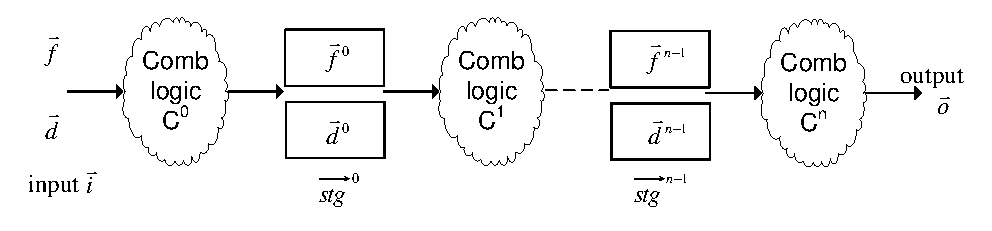
\includegraphics[width=\textwidth]{pipemod1}
\end{center}
\caption{A general structure of the encoder with pipeline stages and flow control mechanism}
  \label{fig_pipeenc}
\end{figure}


Thus,
each $C^j$ can be seen as a small encoder that computes $\vec{stg}^j$ or $\vec{o}$
from $\vec{stg}^{j-1}$ or $\vec{i}$.

In the remainder of this paper,
superscript always means the pipeline stage,
while the subscript,
as mentioned in Subsection \ref{subsec_fsm},
always means the step index in the unrolled transition function.
For example,
$\vec{stg}^j$ is the $j$-th pipeline stage.
While $\vec{stg}^j_i$ is the value of this $j$-th pipeline stage 
at the $i$-th step in the unrolled state transition sequence.

\subsection{Inferring $p$, $l$ and $r$}\label{subsec_inferplr}
Before inferring the pipeline stages,
we first apply the algorithm of \cite{ShenTCAD11} to infer the value of $p$, $l$ and $r$ that can make the 
output sequence $<o_{p},\dots,o_{p+l+r}>$ uniquely determine all $i_{p+l}\in \vec{i}_{p+l}$.
This algorithm iteratively increase a parameter $b$,
and set $p$, $l$ and $r$ all to $b$,
until $F_{PC}(p,l,r)$ become unsatisfiable for all $i_{p+l}\in \vec{i}_{p+l}$.

\subsection{Minimizing $r$ and $l$}\label{reduceing}

\begin{algorithm}[t]
\SetAlgoVlined
\For{$r':=r \to 0$} {
\ShowLnLabel{testr_1}
  \If{$r'\equiv 0$ or $F_{PC}(p,l,r'-1)$ is satisfiable for some $i\in \vec{i}$} {
    break
  }
}
return $r'$
\caption{$RemoveRedundancy(p,l,r)$}
\label{algo_remove2}
\end{algorithm}

As Subsection \ref{subsec_inferplr} increases $p$, $l$ and $r$ simultaneously,
there may be some redundancy in the value of $l$ and $r$.
So we need to first minimize $r$ in Algorithm \ref{algo_remove2}.


% To simplify the presentation,
% we will only introduce the $r$ case.
In Line \ref{testr_1},
when $F_{PC}(p,l,r'-1)$ is satisfiable,
then $r'$ is the last one that makes $F_{PC}(p,l,r')$ unsatisfiable,
we return it directly.
On the other hand,
when $r'\equiv 0$,
$F_{PC}(p,l,0)$ must have been tested in last iteration,
and the result must be unsatisfiable.
In this case we return $0$.

% Minimizing $l$ is similar but with two exceptions:
% First, 
% the range of $l'$ to be enumerated contains some negative value,
% which means $i$ only depend on the value of $o$ in the future.
% Second,
% to be compatible with such cases,
% we use a new formula $F'_{PC}$ in Line \ref{testr_2}.
% When $l\ge 0$,
% $F'_{PC}$ equals to $F_{PC}$.
% But when $l<0$,
% $F'_{PC}$ is define below:
% 
% \begin{multline}\label{uniqt11}
% % \begin{split}
% F'_{PC}(p,l,r):=\\
% \left\{
% \begin{array}{cc}
% &\bigwedge_{m=0}^{p+l+r}
% \{
% (\vec{s}_{m+1},\vec{o}_m)\equiv T(\vec{s}_m,\vec{i}_m)
% \}
% \\
% \wedge&\bigwedge_{m=0}^{p+l+r}
% \{
% (\vec{s'}_{m+1},\vec{o'}_m)\equiv T(\vec{s'}_m,\vec{i'}_m)
% \}
% \\
% \wedge&\bigwedge_{m=p-l}^{p+r}\vec{o}_m\equiv \vec{o'}_m \\
% \wedge& i_{p}\equiv 1 \wedge  i'_{p}\equiv 0 
% % \wedge&\bigwedge_{m=0}^{p+l+r}assertion(\vec{i}_m) \\
% % \wedge&\bigwedge_{m=0}^{p+l+r}assertion(\vec{i'}_m) 
% \end{array}
% \right\}
% % \end{split}
% \end{multline}
% 
% The only change of Equation (\ref{uniqt11}) compared to Equation (\ref{uniqt1})
% are that 
% the range of output vector is change to $p-l\le m\le p+r$,
% while the subscripts of $i$ and $i'$ in the last line refer to $p$ only,
% $l$ are removed.

Now, 
we have a minimized $r$ from Algorithm \ref{algo_remove2},
which can make $\vec{i}_{p+l}$ to be uniquely determined by $<\vec{o}_{p},\dots,\vec{o}_{p+l+r}>$.

\begin{figure}[b]
\begin{center}
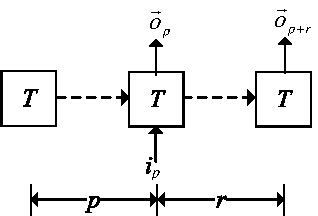
\includegraphics[width=0.5\textwidth]{pc1}
\end{center}
\caption{Recovering input with reduced output sequence}
  \label{fig_pc1}
\end{figure}

We further require that :
\begin{enumerate}
 \item As shown in Figure \ref{fig_pc1},
 $l$ can be reduced to 0,
 which means $\vec{i}_{p}$ can be uniquely determined by $<\vec{o}_{p},\dots,\vec{o}_{p+r}>$,
 that is,
 the set of future outputs.
 \item The above mentioned output sequence $<\vec{o}_{p},\dots,\vec{o}_{p+r}>$ 
 can be further reduced to $\vec{o}_{p+r}$.
 This means $\vec{o}_{p+r}$ is the only output vector needed to recover the input vector $\vec{i}_p$.
\end{enumerate}

Checking these two requirements
equals to checking the unsatisfiability of the following equation.

\begin{equation}\label{uniqt11}
% \begin{split}
F'_{PC}(p,r):=
\left\{
\begin{array}{cc}
&\bigwedge_{m=0}^{p+r}
\{
(\vec{s}_{m+1},\vec{o}_m)\equiv T(\vec{s}_m,\vec{i}_m)
\}
\\
\wedge&\bigwedge_{m=0}^{p+r}
\{
(\vec{s'}_{m+1},\vec{o'}_m)\equiv T(\vec{s'}_m,\vec{i'}_m)
\}
\\
\wedge&\vec{o}_{p+r}\equiv \vec{o'}_{p+r} \\
\wedge& i_{p}\equiv 1 \wedge  i'_{p}\equiv 0 
% \wedge&\bigwedge_{m=0}^{p+l+r}assertion(\vec{i}_m) \\
% \wedge&\bigwedge_{m=0}^{p+l+r}assertion(\vec{i'}_m) 
\end{array}
\right\}
% \end{split}
\end{equation}


This equation seems much stronger than the general requirement in Equation (\ref{uniqt1}).
But we will show in experimental results that 
they are always fulfilled.



\subsection{Inferring pipeline stages}\label{subsec_inferstage}

Now,
with the inferred $p$ and $r$,
we need to generalize $F'_{PC}$ in Equation (\ref{uniqt11}) to the following new formula that
can determine whether a particular variable $v$ at step $j$
can be uniquely determined by a vector $\vec{w}$ at step $k$.
Now $v$ and $\vec{w}$ can be either input, registers or output variables.

\begin{equation}\label{uniqt2}
% \begin{split}
F''_{PC}(p,r,v,j,\vec{w},k):=
\left\{
\begin{array}{cc}
&\bigwedge_{m=0}^{p+r}
\{
(\vec{s}_{m+1},\vec{o}_m)\equiv T(\vec{s}_m,\vec{i}_m)
\}
\\
\wedge&\bigwedge_{m=0}^{p+r}
\{
(\vec{s'}_{m+1},\vec{o'}_m)\equiv T(\vec{s'}_m,\vec{i'}_m)
\}
\\
\wedge&\vec{w}_{k}\equiv \vec{w'}_{k} \\
\wedge& v_{j}\equiv 1 \wedge  v'_{j}\equiv 0 
% \wedge&\bigwedge_{m=0}^{p+l+r}assertion(\vec{i}_m) \\
% \wedge&\bigwedge_{m=0}^{p+l+r}assertion(\vec{i'}_m) 
\end{array}
\right\}
% \end{split}
\end{equation}

Obviously,
when $F''_{PC}(p,r,v,j,\vec{w},k)$ is unsatisfiable,
$\vec{w}_k$ can uniquely determine $v_j$.

The last pipeline stage $\vec{stg}^{n-1}$ is 
exactly the set of registers $s\in \vec{s}$ 
that can be uniquely determined at the $p+r$-th step by $\vec{o}$.
% With Equation (\ref{uniqt2}),
It can be formally defined as:

\begin{equation}\label{stgn_1}
 \vec{stg}^{n-1} := 
\left\{
 s\in \vec{s} ~| 
% \begin{array}{cc}
 F''_{PC}(p,r,
 s,p+r,
 \vec{o},p+r)
 ~is~unsatisfiable
% \end{array}
\right\}
\end{equation}

% And the second to last pipeline stage $\vec{stg}^{n-2}$ 
% is exactly the set of registers $s\in \vec{s}/\vec{stg}^{n-1}$
% that can be uniquely determined at the $p+r-1$-th step by $\vec{stg}^{n-1}$ at $p+r$-th step.
% 
% \begin{multline}\label{stgn_2}
%  \vec{stg}^{n-2} := \\
%  \left\{
%  s\in \vec{s}/\vec{stg}^{n-1} ~| 
% \begin{array}{cc}
%  F''_{PC}(p,r,s,p+r-1,\vec{stg}^{n-1},p+r)\\
%  ~is~unsatisfiable
% \end{array}
% \right\}
% \end{multline}

Similarly,
for $0\le j\le n-2$,
$\vec{stg}^j$ at $j-((n-2)-(p+r-1))$-th step
can be uniquely determined by $\vec{stg}^{j+1}$ at $j-((n-2)-(p+r-1))+1$-th step.
So we can recursively defined $\vec{stg}^j$ as :

\begin{equation}\label{stgn_def}
\begin{array}{ccc}
S             & := & \vec{s}/\bigcup_{j<k\le n-2}\vec{stg}^{k}\\
D             & := & (n-2)-(p+r-1)\\
\end{array}
\end{equation}

\begin{equation}\label{stgn_j}
\vec{stg}^{j} := 
 \left\{
 s\in S ~| 
% \begin{array}{cc}
 F''_{PC}(p,r,s,j-D,\vec{stg}^{j+1},j-D+1)
 ~is~unsatisfiable
% \end{array}
\right\}
\end{equation}

With Equation (\ref{stgn_1}) and (\ref{stgn_j}),
all the pipeline stages can now be inferred.

\subsection{Inferring the pipeline stage that uniquely determines input vector}\label{subsec_inferinput}

According to Figure \ref{fig_pipeenc},
$\vec{stg}^0$ defined in Equation (\ref{stgn_j}) is
exactly the pipeline stage that uniquely determined the input vector $\vec{i}$.

But in real encoders,
this may not be the case.
So we need to search for the smallest $j$ from $0$ to $n-1$ that can make $\vec{i}$ to be uniquely determined by $\vec{stg}^j$,
that is,
the smallest $j$ that can make $F''_{PC}(p,r,i,p,\vec{stg}^{j},j-D)$ unsatisfiable for all $i\in \vec{i}$,
with $D$ defined in Equation (\ref{stgn_def}).

\subsection{Finding out the flow control vectors in each pipeline stage}

\section{Characterizing the Boolean function of input variables and pipeline registers}\label{sec_char}
\subsection{Characterizing the Boolean function of the last pipeline stage}

According to Equation (\ref{stgn_1}),
every registers $s\in \vec{stg}^{n-1}$ can be uniquely determined by $\vec{o}$ at the $p+r$-th step,
that is,
$F''_{PC}(p,r,s,p+r,\vec{o},p+r)$ is unsatisfiable and can be partitioned into :

\begin{equation}
 \phi_A := 
 \left\{
\begin{array}{cc}
&\bigwedge_{m=0}^{p+r}
\{
(\vec{s}_{m+1},\vec{o}_m)\equiv T(\vec{s}_m,\vec{i}_m)
\}
\\
\wedge& s_{p+r}\equiv 1 
\end{array}
\right\}
\end{equation}

\begin{equation}
% \begin{split}
\phi_B := 
\left\{
\begin{array}{cc}
&\bigwedge_{m=0}^{p+r}
\{
(\vec{s'}_{m+1},\vec{o'}_m)\equiv T(\vec{s'}_m,\vec{i'}_m)
\}
\\
\wedge&\vec{o}_{p+r}\equiv \vec{o'}_{p+r} \\
\wedge& s'_{p+r}\equiv 0 
% \wedge&\bigwedge_{m=0}^{p+l+r}assertion(\vec{i}_m) \\
% \wedge&\bigwedge_{m=0}^{p+l+r}assertion(\vec{i'}_m) 
\end{array}
\right\}
% \end{split}
\end{equation}

As $F''_{PC}(p,r,s,p+r,\vec{o},p+r)$ equals to $\phi_A \wedge \phi_B$,
so $\phi_A \wedge \phi_B$ is unsatisfiable.
And the common variables of $\phi_A$ and $\phi_B$ is $\vec{o}_{p+r}$.

According to \cite{InterpBoolFunction},
a Craig interpolant $\phi_I$ of $\phi_A$ with respect to $\phi_B$ can be constructed,
which refer only to $\vec{o}_{p+r}$,
and covers all the valuation of $\vec{o}_{p+r}$ that can make $s_{p+r}\equiv 1$.
At the same time,
$\phi_I\wedge \phi_B$ is unsatisfiable,
which means $\phi_I$ covers nothing that can make $s_{p+r}\equiv 0$.

Thus,
$\phi_I$ can be used as the decoder's Boolean function that recovers $s\in \vec{stg}^{n-1}$ from $\vec{o}$.

\subsection{Characterizing the Boolean function of other pipeline stages}
Similar to last subsection,
we can partition the unsatisfiable formula $F''_{PC}(p,r,s,j-D,\vec{stg}^{j+1},j-D+1)$ 
in Equation (\ref{stgn_j}) into the following two equations:

\begin{equation}
 \phi_A := 
 \left\{
\begin{array}{cc}
&\bigwedge_{m=0}^{p+r}
\{
(\vec{s}_{m+1},\vec{o}_m)\equiv T(\vec{s}_m,\vec{i}_m)
\}
\\
\wedge& s_{j-D}\equiv 1 
\end{array}
\right\}
\end{equation}

\begin{equation}
% \begin{split}
\phi_B := 
\left\{
\begin{array}{cc}
&\bigwedge_{m=0}^{p+r}
\{
(\vec{s'}_{m+1},\vec{o'}_m)\equiv T(\vec{s'}_m,\vec{i'}_m)
\}
\\
\wedge&\vec{stg}^{j+1}_{j-D+1}\equiv \vec{stg'}^{j+1}_{j-D+1} \\
\wedge& s'_{j-D}\equiv 0 
% \wedge&\bigwedge_{m=0}^{p+l+r}assertion(\vec{i}_m) \\
% \wedge&\bigwedge_{m=0}^{p+l+r}assertion(\vec{i'}_m) 
\end{array}
\right\}
% \end{split}
\end{equation}

Again,
a Craig interpolant $\phi_I$ of $\phi_A$ with respect to $\phi_B$ can be constructed,
and used as the decoder's Boolean function that recovers $s\in \vec{stg}^{j}$ from $\vec{stg}^{j+1}$.

\subsection{Characterizing the Boolean function of the encoder's input variables}

According to Subsection \ref{sec_pipeinfer}.\ref{subsec_inferinput},
we have found the smallest $j$ that can make $F''_{PC}(p,r,i,p,\vec{stg}^{j},j-D)$ unsatisfiable for all $i\in \vec{i}$,
with $D$ defined in Equation (\ref{stgn_def}).
$F''_{PC}(p,r,i,p,\vec{stg}^{j},j-D)$ is unsatisfiable and can be partitioned into :

\begin{equation}
% \begin{split}
\phi_A:=
\left\{
\begin{array}{cc}
&\bigwedge_{m=0}^{p+r}
\{
(\vec{s}_{m+1},\vec{o}_m)\equiv T(\vec{s}_m,\vec{i}_m)
\}
\\
\wedge& i_{p}\equiv 1 
% \wedge&\bigwedge_{m=0}^{p+l+r}assertion(\vec{i}_m) \\
% \wedge&\bigwedge_{m=0}^{p+l+r}assertion(\vec{i'}_m) 
\end{array}
\right\}
% \end{split}
\end{equation}

\begin{equation}
% \begin{split}
\phi_B:=
\left\{
\begin{array}{cc}
&\bigwedge_{m=0}^{p+r}
\{
(\vec{s'}_{m+1},\vec{o'}_m)\equiv T(\vec{s'}_m,\vec{i'}_m)
\}
\\
\wedge&\vec{stg}^j_{j-D}\equiv \vec{stg'}^j_{j-D} \\
\wedge& i'_{p}\equiv 0 
% \wedge&\bigwedge_{m=0}^{p+l+r}assertion(\vec{i}_m) \\
% \wedge&\bigwedge_{m=0}^{p+l+r}assertion(\vec{i'}_m) 
\end{array}
\right\}
% \end{split}
\end{equation}

Similar to last subsection,
the Craig interpolant $\phi_I$ of $\phi_A$ with respect to $\phi_B$ 
can be used as the decoder's Boolean function that recovers $i\in\vec{i}$ from $\vec{stg}^j$.













\section{Experimental results}\label{sec_exp}
\subsection{The usage model}
All these steps mentioned above are connected together by the standard make tool in Linux.
To use the synthesis mode,
the user needs to run the command "make halting" under the bash shell in the benchmark directory.
To use the inferring mode,
the user needs to run the command "make infer\_multidec\_not\_charfirst \_nowall".

\subsection{Benchmarks}
The benchmarks used in the experiments include several complex encoders from industrial projects,
\begin{enumerate}
\item A XGXS encoder compliant to clause 48 of IEEE-802.3ae 2002 standard .
\item A XFI encoder compliant to clause 49 of the same IEEE standard.
\item A 66-bit scrambler used to ensure
that a data sequence has sufficient 0-1 transitions,
so that it can run through a high-speed
noisy serial transmission channel.
\item A PCI-E physical coding module .
\item The Ethernet module of Sun's OpenSparc T2 processor.
\end{enumerate}

The profiles of these benchmarks are shown in Table \ref{tab_benchmark}.
Some of these large benchmarks have more than 1000 lines of source code,
while the XFI encoder has more than 100 state variables and configuration pins.


\begin{table}[t]
\centering
\caption{Information on Benchmarks}
\begin{tabular}{|c|c|c|c|c|c|}
\hline
&XGXS&XFI&scrambler&PCIE&T2 Ethernet\\\hline\hline
Line number&&&&&\\
of verilog&214&466&24&1139&1073\\
source code&&&&&\\\hline
\#state variables&15&135&58&22&48\\\hline
Data path width&8&64&66&10&10\\\hline
\end{tabular}\label{tab_benchmark}
\end{table}

\subsection{The experimental result of the synthesis mode}
\begin{table}[t]
\centering
\caption{Experimental results on the correct and incorrect encoders}
\begin{tabular}{|c|c|c|c|c|c|c|}
\hline
&                                        &XGXS     &XFI       &scrambler     &PCI-E    &T2 Ethernet\\ \hline\hline
% &Time to ch-                           &&&&&\\
% 
% &$d,p,l$                                 &1,1,1    &0,3,2     &0,2,2     &2,1,1   &4,1,1         \\ \hline\hline
For &Time to check the                         &&&&&\\
correct&decoder's existence(sec)                      &0.29     &17.86     &2.67      &0.47    &29.64\\\cline{2-7}
%      &improve \%                         &72.64    &74.67     &53.48     &80.42   &55.34 \\\cline{2-7}
encoder&$d,p,l$                                 &1,2,1    &0,3,2     &0,2,2     &2,2,1   &4,4,1          \\ \hline\hline
For&Time to check the                          &&&&&\\
incorrect&decoder's existence(sec)             &0.16     &7.59     &1.17      &0.33    &2.19\\
encoder&                        &&&&&\\\hline

\end{tabular}\label{tab_prodes}
\end{table}

According to Table \ref{tab_prodes} and ,
when given the assertion,
%no matter correct or not,
the synthesis mode can determine the existence of the decoders within 40 seconds,
and builds the decoders within 10 seconds with an algorithm similar to that of Liu et al. .

Moreover,
we inserted some bugs into these encoders,
which generated the same output letter for two different input letters.
CompSyn successfully detected all these bugs within 10 seconds.

\subsection{The experimental result of the inferring mode}
\begin{table}[b]
\centering
\caption{Experimental Results of the inferring mode}
\begin{tabular}{|c|c|c|c|c|c|c|}
\hline
                                        &XGXS     &XFI       &scrambler     &PCI-E    &T2 Ethernet\\\hline\hline
Config                 &&&&&\\
pin number                              &3        &120       &1             &16      &26\\\hline
Runtime                                 &3.83     &3841.34   &18.73         &8.51    &1791.22      \\\hline
$d,p,l$                                 &1,5,1    &0,5,2     &0,4,2         &2,5,1   &4,5,1          \\ \hline
Number of                               &&&&&          \\
decoders                                &1        &2         &2             &1       &1          \\ \hline
\end{tabular}\label{tab_res}
\end{table}

According to Table 	\ref{tab_res},
when the assertions are not known,
the inferring mode can infer assertions, generate decoders and infer these decoders' precondition formulas within 4000 seconds.

The set of inferred assertions are shown below:

\textbf{For XGXS}:
\texttt{( ( !bad\_code ) )}

\textbf{For XFI}:
\texttt{( ( TEST\_MODE ) | ( !TEST\_MODE \& RESET ) | ( !TEST\_MODE \& !RESET \& DATA\_VALID ) )}

\textbf{For scrambler}:
\texttt{True}

\textbf{For PCI-E}:
\texttt{( ( !TXELECIDLE \& CNTL\_TXEnable\_P0 \& CNTL\_RESETN\_P0 \& !CNTL\_Loopback\_P0 ) )}

\textbf{For T2 ethernet}:
\texttt{( ( link\_up\_loc \& !reset\_tx \& !txd\_sel[1] \& !jitt er\_study\_pci[1] \& !txd\_sel[0] \& !jitter\_study\_pci[0] ) | ( !link\_up\_l oc \& !reset\_tx \& !txd\_sel[1] \& tx\_enc\_conf\_sel[3] \& tx\_enc\_conf\_sel[2] \& !jitter\_study\_pci[1] \& !txd\_sel[0] \& !jitter\_study\_pci[0] ) | ( !l ink\_up\_loc \& !reset\_tx \& !txd\_sel[1] \& tx\_enc\_conf\_sel[3] \& !tx\_enc\_conf \_sel[2] \& tx\_enc\_conf\_sel[1] \& !jitter\_study\_pci[1] \& !txd\_sel[0] \& !ji tter\_study\_pci[0] ) | ( !link\_up\_loc \& !reset\_tx \& !txd\_sel[1] \& !tx\_ enc\_conf\_sel[3] \& !tx\_enc\_conf\_sel[2] \& tx\_enc\_conf\_sel[1] \& !jitter\_ study\_pci[1] \& !txd\_sel[0] \& !jitter\_study\_pci[0] \& tx\_enc\_conf\_sel[0] ) )}

Moreover,
only two out of the five benchmarks have two decoders,
while the other three have only one decoder.
This means that,
in most cases,
our algorithm generates only one decoder.
For other cases with multiple decoders,
the user needs to inspect the inferred precondition formulas to select the correct one.

For the two decoders of scrambler,
their corresponding precondition formulas are $reset$ and $!reset$.
By inspecting the Verilog source code of scrambler,
we found that the $reset$ is used to reset the scrambler when it is $True$.
Thus,
the scrambler encoder will work in normal mode when $reset$ is $False$.
Therefore,
the second decoder is the correct one.
And the dynamic simulation had confirmed its correctness.


For the two decoders of the most complex XFI encoder ,
their corresponding precondition formulas are $RESET~\& !TEST\_MODE~\&~!DATA\_VALID$ and $!RESET~\&~!TEST\_MODE~\&~DATA\_VALID$.
The only differences between them are the value of $RESET$ and $DATA\_VALID$.
By inspecting the Verilog source code of XFI,
we found that the $RESET$ is used to reset the XFI encoder when it is $True$,
and $DATA\_VALID$ means that the input data is valid when it is $True$.
So,
the XFI encoder will work in normal mode when $RESET$ is $False$ and $DATA\_VALID$ is $True$.
Therefore,
the second decoder is the correct one.
The dynamic simulation had also confirmed its correctness.

In this process,
the user only needs to inspect the meaning of two configuration pins,
instead of all 120 configuration pins of the XFI encoder.
In this way,
the human effort in specifying assertion and selecting the correct decoder is significantly reduced.

\section{Conclusions}\label{sec_conclude}
The CompSyn tool can infer correct assertions and generate decoder circuits for several complex encoders.
Furthermore,
it can significantly reduce the human effort in specifying assertion and selecting the correct decoder.


% \section*{Acknowledgment}
% The authors would like to thank the anonymous reviewers for their hard work.

% This work was funded by Projects 60603088 and 61070132 supported by National Natural Science Foundation of China.


\bibliographystyle{abbrv}
\bibliography{ssy}


% \begin{thebibliography}{4}
% 
% \end{thebibliography}



\end{document}
